\section{Resultados}

Se presentan los resultados obtenidos en el pronóstico del tipo de cambio utilizando el modelo de caminata aleatoria y los modelos monetarios, en su versión lineal y a través de redes neuronales artificiales de ocho y nueve neuronas.

\subsection{Modelo de caminata aleatoria}
Utilizando la serie de tipo de cambio, se utilizan 144 observaciones mensuales (desde enero de 2001 hasta diciembre de 2013) para pronosticar el tipo de cambio 36 períodos adelante (desde enero de 2013 hasta diciembre de 2015).

\subsubsection{Pronóstico fuera de la muestra}

\begin{figure}[htb]
	\centering
	\caption{Pronóstico del tipo de cambio Q/USD con modelo de caminata aleatoria}
	\label{fig:rwout}
	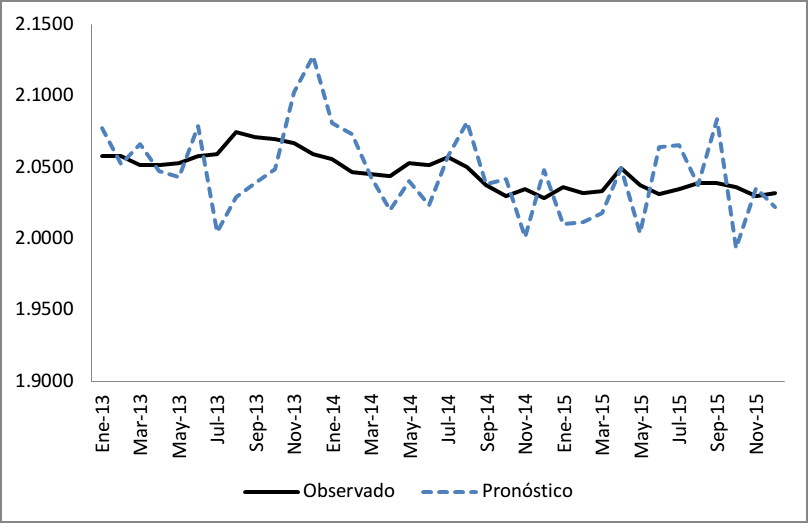
\includegraphics[width=0.9\textwidth]{figuras/RW_out.png}
	\caption*{Fuente: elaboración propia.}
\end{figure}

\clearpage
%\vspace*{1cm}
En la figura \ref{fig:rwout} se muestra el pronóstico del tipo de cambio. Como se puede observar, los valores pronosticados del tipo de cambio siguen la tendencia del tipo de cambio observado.\\

Las medidas de error obtenidas son relativamente pequeñas (RMSE = 0.0276 y RMSPE = 0.0135). Además, el modelo captura correctamente un PERC = 42\% de los puntos de inflexión respecto al aumento o disminución del tipo de cambio en el siguiente período.\\

Finalmente, se puede decir que el modelo presenta mucha volatilidad alrededor de la tendencia del tipo de cambio observado. Esto es debido a que la varianza utilizada para generar la componente aleatoria $\epsilon_t$ del modelo se ve afectada significativamente a inicios de los años 2000 y durante los años 2008 a 2011.

\newpage
\subsection{Modelo monetario lineal}
Utilizando los resultados de un modelo de regresión lineal obtenidos con EViews 9 se obtienen los valores ajustados del tipo de cambio dentro de la muestra de estimación, y los pronósticos del tipo de cambio.\\

En la tabla \ref{tab:estimlin} se muestra la estimación para el modelo monetario lineal. Como se observa, tanto la oferta de dinero, como la inflación no resultan estadísticamente significativas. Asimismo, los signos de la oferta monetaria, el ingreso real, y la tasa de interés no son los esperados de acuerdo con el modelo teórico. Y de acuerdo con el modelo teórico de precios rígidos, la velocidad de ajuste de las desviaciones del tipo de cambio resulta negativa.

\input{tablas/regLineal}

En la estimación del modelo se obtuvo el problema de autocorrelación de los errores, pero debido a que el enfoque de este trabajo consiste en evaluar el desempeño de los modelos de pronóstico, no se realiza ninguna modificación en la estimación del modelo.

\subsubsection{Pronóstico dentro de la muestra}
Utilizando los resultados obtenidos del modelo monetario lineal, se utilizan para obtener los valores ajustados dentro de la muestra. En la figura \ref{fig:linin} se muestra el pronóstico dentro de la muestra para el tipo de cambio.\\

\begin{figure}[htb]
	\centering
	\caption{Ajuste del tipo de cambio Q/USD con modelo monetario lineal}
	\label{fig:linin}
	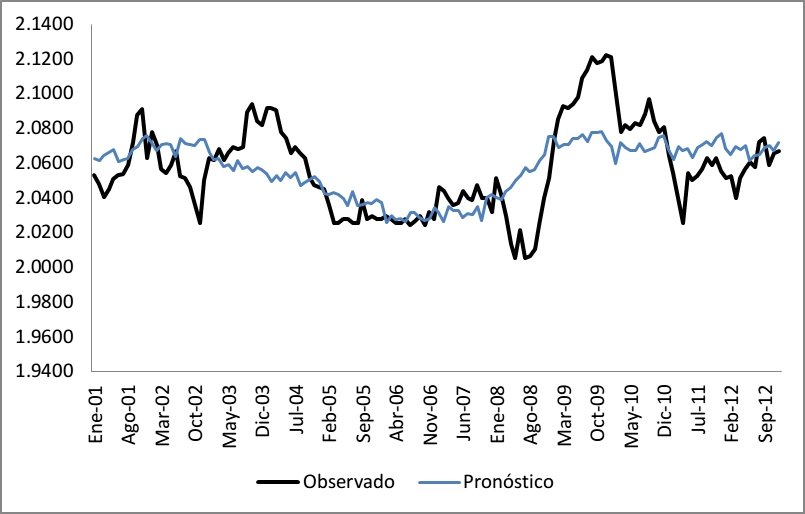
\includegraphics[width=0.7\textwidth]{figuras/lin_in.png}
	\caption*{Fuente: elaboración propia.}
\end{figure}

Como se observa, el modelo monetario lineal se ajusta suavemente a la tendencia del tipo de cambio observado durante el período de estimación, y en general, este no puede explicar las fuertes desviaciones de la tendencia. Respecto a las medidas de error, se obtienen valores relativamente pequeños (RMSE = 0.0208 y RMSPE = 0.0101), y además se obtiene porcentaje de predicción de puntos de inflexión PERC = 55\% de las observaciones dentro de la muestra.

\newpage
\subsubsection{Pronóstico fuera de la muestra}
Con la estimación del modelo se procede a obtener el pronóstico del tipo de cambio, el cual se muestra en la figura \ref{fig:linout}. Como se puede observar, dicho pronóstico sigue una tendencia relativamente constante y no logra percibir la caída del tipo de cambio a partir de septiembre de 2013.\\

\begin{figure}[htb]
	\centering
	\caption{Pronóstico del tipo de cambio Q/USD con modelo monetario lineal}
	\label{fig:linout}
	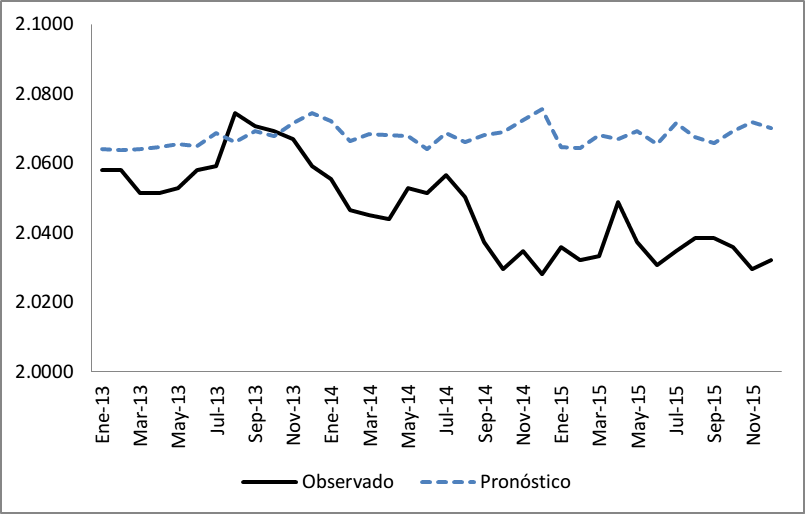
\includegraphics[width=0.7\textwidth]{figuras/lin_out.png}
	\caption*{Fuente: elaboración propia.}
\end{figure}

En cuanto a las medidas de error, presenta menores valores que el modelo de caminata aleatoria (RMSE = 0.0251 y RMSPE = 0.0123) y una mayor tasa de predicción de puntos de inflexión (PERC = 43\% de 36 observaciones fuera de la muestra).

\clearpage

\subsection{Modelo monetario de RNA con 8 neuronas}
Se ajusta una RNA de una capa oculta con ocho neuronas utilizando las variables normalizadas como se menciona en la metodología. 
% Esto va en la metodología
Asimismo, la elección de la arquitectura de la red neuronal se decide por las medidas de error de pronóstico, tanto adentro como afuera de la muestra.

\subsubsection{Pronóstico dentro de la muestra}
En la figura \ref{fig:annin18} se muestran los valores pronosticados dentro de la muestra para el tipo de cambio. Se puede observar que la red neuronal aprende sobresalientemente ($R^2 = 0.91$) el patrón de comportamiento del tipo de cambio dentro de la muestra de entrenamiento. Asimismo, exhibe medidas de error más bajas que las del modelo de caminata aleatoria y del modelo lineal (RMSE = 0.0076 y RMSPE = 0.0037). Y finalmente, logra predecir correctamente un 72\% (sobre las 144 observaciones) de los puntos de inflexión de la muestra.

\begin{figure}[htb]
	\centering
	\caption{Ajuste del tipo de cambio Q/USD con modelo de RNAs 8 neuronas}
	\label{fig:annin18}
	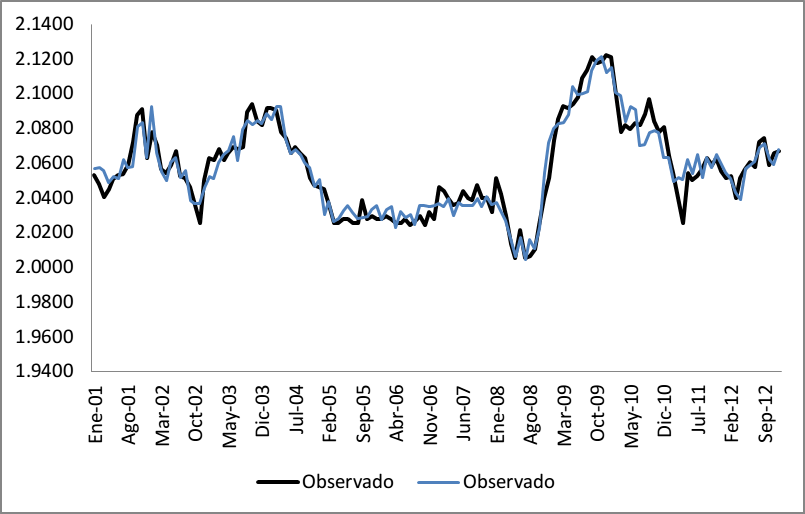
\includegraphics[width=0.7\textwidth]{figuras/ann18_in.png}
	\caption*{Fuente: elaboración propia.}
\end{figure}

\subsubsection{Pronóstico fuera de la muestra}

En la figura \ref{fig:annout18} se muestra el pronóstico de la red neuronal utilizando valores fuera de la muestra de entrenamiento. Como se puede observar, la red neuronal predice con mejor precisión la volatilidad en el tipo de cambio porque aprende el patrón de movimiento de las variables, lo que lleva a una mejor predicción del tipo de cambio. Y aunque existe un sesgo de nivel en la predicción del modelo sobre el tipo de cambio observado, la red neuronal consigue un balance entre la explicación de la volatilidad y el nivel del tipo de cambio. 

\begin{figure}[htb]
	\centering
	\caption{Pronóstico del tipo de cambio Q/USD con modelo de RNAs 8 neuronas}
	\label{fig:annout18}
	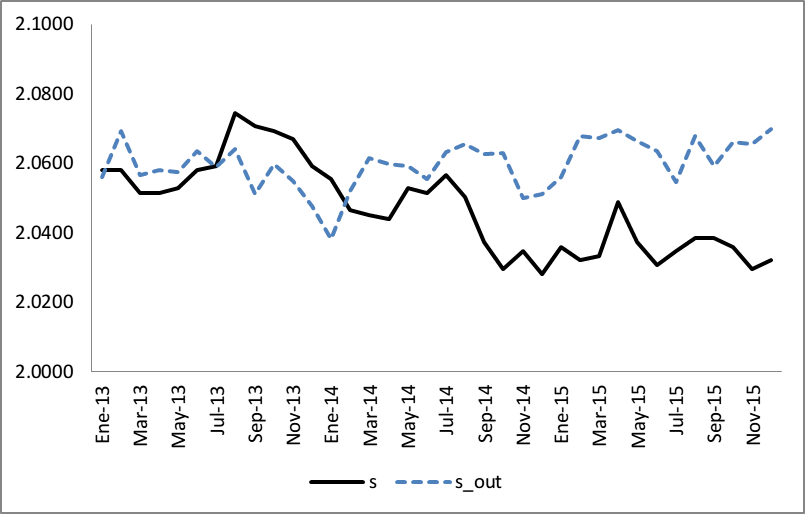
\includegraphics[width=0.7\textwidth]{figuras/ann18_out.png}
	\caption*{Fuente: elaboración propia.}
\end{figure}

En cuanto a las medidas de error, el pronóstico fuera de la muestra exhibe menores indicadores que el modelo lineal y el modelo de caminata aleatoria (RMSE = 0.02059 y RMSPE = 0.01011). Y en cuanto al pronóstico de puntos de inflexión, logra predecir un 57\% sobre las 36 observaciones fuera de la muestra, porcentaje que es mayor al indicador obtenido por el modelo lineal y el de caminata aleatoria.



\subsection{Modelo monetario de RNA con 9 neuronas}
Se repite el experimento de entrenamiento de una RNA con una capa oculta y nueve neuronas.

\subsubsection{Pronóstico dentro de la muestra}
En la figura \ref{fig:annin19} se muestran los valores pronosticados dentro de la muestra para el tipo de cambio. Nuevamente, la red neuronal se ajusta extraordinariamente ($R^2 = 0.92$) al patrón de comportamiento del tipo de cambio dentro de la muestra de entrenamiento. Asimismo, exhibe medidas de error más bajas que las del modelo de caminata aleatoria y del modelo lineal (RMSE = 0.0070 y RMSPE = 0.0034). Y finalmente, logra predecir correctamente un 73\% (sobre las 144 observaciones) de los puntos de inflexión de la muestra. En comparación con la red neuronal de ocho neuronas, este modelo se desempeña ligeramente mejor en las medidas de error de pronóstico, y relativamente peor en la predicción correcta de puntos de inflexión.

\begin{figure}[htb]
	\centering
	\caption{Ajuste del tipo de cambio Q/USD con modelo de RNAs 9 neuronas}
	\label{fig:annin19}
	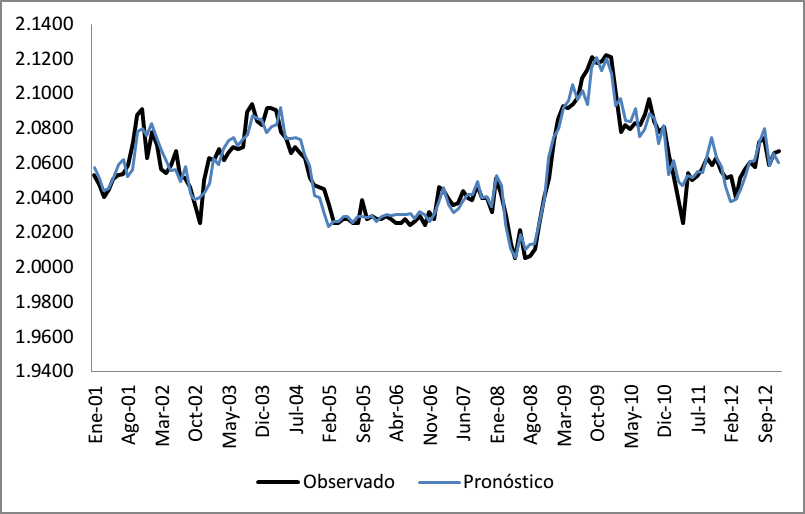
\includegraphics[width=0.7\textwidth]{figuras/ann19_in.png}
	\caption*{Fuente: elaboración propia.}
\end{figure}


\subsubsection{Pronóstico fuera de la muestra}

En la figura \ref{fig:annout19} se muestra el pronóstico de la red neuronal utilizando valores fuera de la muestra de entrenamiento. Como se puede observar, la red neuronal predice con mejor precisión la volatilidad en el tipo de cambio porque aprende el patrón de movimiento de las variables, lo que lleva a una mejor predicción del tipo de cambio. Y aunque existe un sesgo de nivel en la predicción del modelo sobre el tipo de cambio observado, la red neuronal consigue un balance entre la explicación de la volatilidad y el nivel del tipo de cambio. 

\begin{figure}[htb]
	\centering
	\caption{Pronóstico del tipo de cambio Q/USD con modelo de RNAs 9 neuronas}
	\label{fig:annout19}
	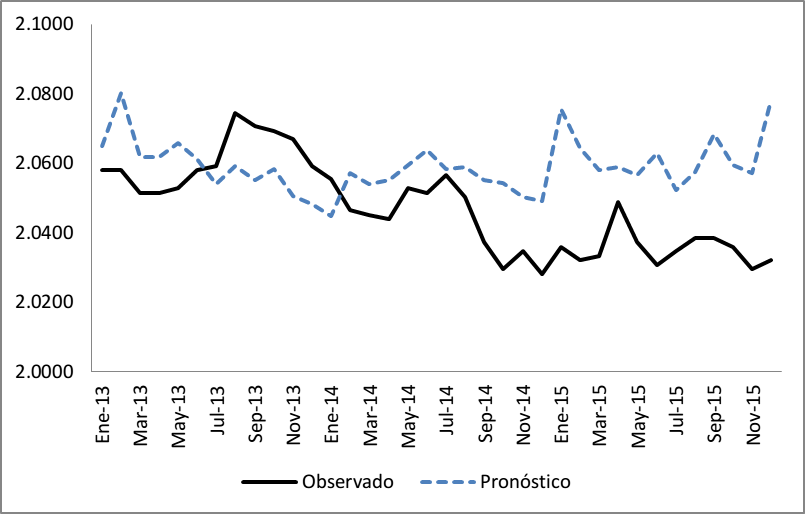
\includegraphics[width=0.7\textwidth]{figuras/ann19_out.png}
	\caption*{Fuente: elaboración propia.}
\end{figure}

En cuanto a las medidas de error, el pronóstico fuera de la muestra exhibe menores indicadores que el modelo lineal y el modelo de caminata aleatoria (RMSE = 0.01969 y RMSPE = 0.00966). Y en cuanto al pronóstico de puntos de inflexión, logra predecir un 46\% sobre las 36 observaciones fuera de la muestra, porcentaje que es mayor al indicador obtenido por el modelo lineal y el de caminata aleatoria.


\subsection{Importancia relativa de variables}
En la figura \ref{fig:importrel18} se muestra el gráfico de importancia relativa para cada una de las variables explicativas del modelo con nueve neuronas, donde \textit{m} representa la oferta relativa de dinero, \textit{i} el diferencial de tasas de interés, \textit{y} el diferencial de ingreso real e \textit{inf} el diferencial de inflación esperada.

\begin{figure}[htb]
	\centering
	\caption{Importancia relativa en el modelo de RNAs con 8 neuronas}
	\label{fig:importrel18}
	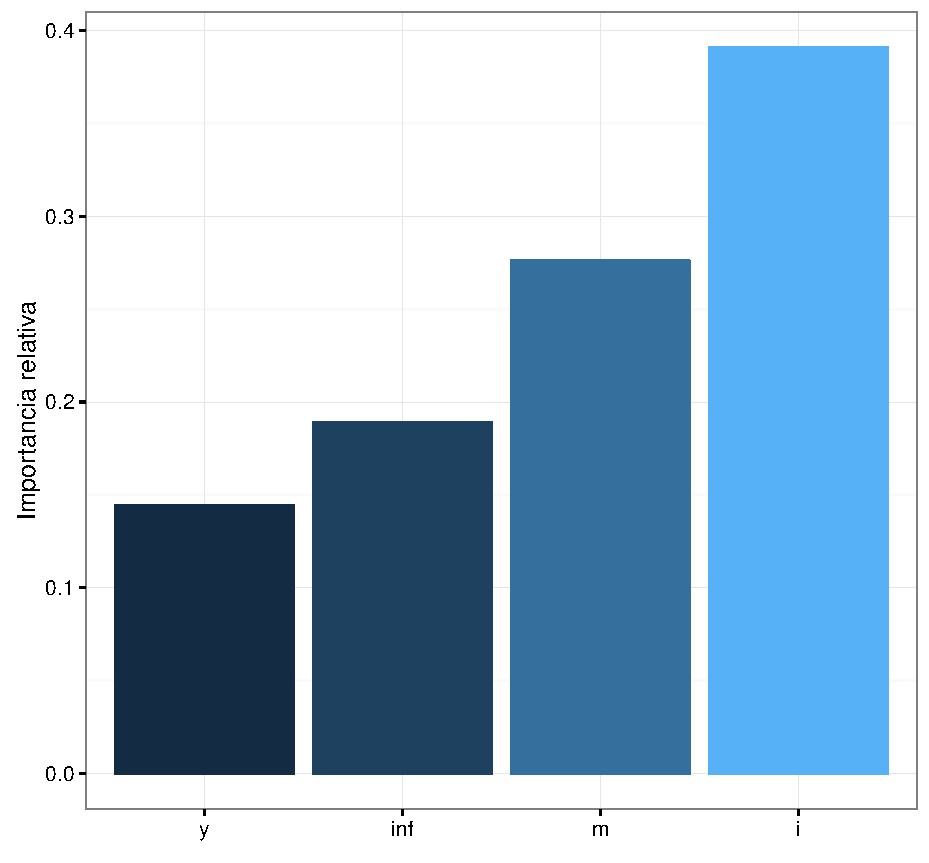
\includegraphics[width=0.6\textwidth]{figuras/garson_18.pdf}
	\caption*{Fuente: elaboración propia.}
\end{figure}

De acuerdo con la importancia relativa de Garson, el ingreso real y la inflación contribuyen muy poco en la explicación del tipo de cambio, mientras que la oferta relativa de dinero y el diferencial de tasas de interés tienen un impacto más significativo sobre el tipo de cambio.\\

\newpage
En la figura \ref{fig:importrel19} se muestra el gráfico de importancia relativa para la red neuronal con nueve neuronas en la capa oculta. Como se puede observar, se reafirma la contribución significativa del diferencial de tasas de interés y de la oferta relativa de dinero.

\begin{figure}[htb]
	\centering
	\caption{Importancia relativa en el modelo de RNAs con 9 neuronas}
	\label{fig:importrel19}
	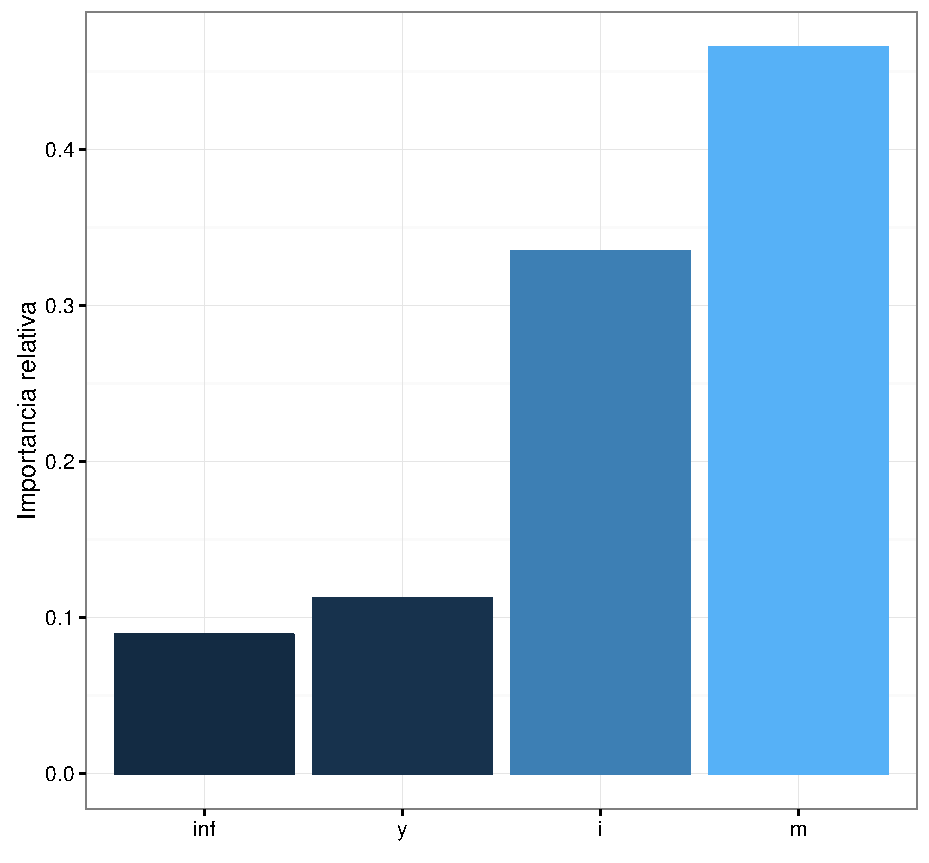
\includegraphics[width=0.6\textwidth]{figuras/garson_19.pdf}
	\caption*{Fuente: elaboración propia.}
\end{figure}

\clearpage
\subsection{Análisis de resultados}
De acuerdo con las medidas de error de pronóstico obtenidas para cada uno de los modelos, como se resumen en la tabla \ref{tab:resOutOfSample}, ambos modelos de redes neuronales proveen un mejor pronóstico en magnitud que los modelos de caminata aleatoria y el modelo lineal, en concordancia con los criterios de RMSE y RMSPE.\\

% Table generated by Excel2LaTeX from sheet 'Tablas'
\begin{table}[htbp]
  \centering
  \caption{Resultados de pronóstico del tipo de cambio Q/USD}
    \begin{tabular}{lrrr}
    \toprule
    \multicolumn{1}{c}{\textbf{Fuera de la muestra}} & \multicolumn{1}{c}{\textbf{RMSE}} & \multicolumn{1}{c}{\textbf{RMSPE}} & \multicolumn{1}{c}{\textbf{PERC}} \\
    \midrule
    Caminata aleatoria    & 0.02763 & 0.01347 & 31\% \\
    Modelo lineal & 0.02512 & 0.01234 & 43\% \\
    RNA con 8 neuronas & 0.02059 & 0.01011 & 57\% \\
    RNA con 9 neuronas & 0.01969 & 0.00966 & 46\% \\
    \bottomrule
    \end{tabular}%
    \caption*{Fuente: elaboración propia.}
  \label{tab:resOutOfSample}%
\end{table}%


En cuanto a la predicción de puntos de inflexión, el modelo monetario lineal supera al de caminata aleatoria, y asimismo, los modelos de RNAs exhiben porcentajes más altos que los del modelo lineal, siendo superior el modelo que utiliza ocho neuronas en la capa oculta.\\

En la tabla \ref{tab:ratioError} se muestra el resumen del cociente de error entre los modelos monetarios y el modelo de caminata aleatoria. Como se puede observar, tanto el modelo monetario lineal como el modelo de redes neuronales poseen una relación de error menor a 1, lo que indica que el modelo de caminata aleatoria posee el peor desempeño de pronóstico del tipo de cambio del quetzal. Es decir, este resultado apoya la hipótesis de que la predicción del tipo de cambio sí se puede llevar a cabo con los fundamentos macroeconómicos, y que toda la información disponible en la serie del tipo de cambio no es suficiente para pronosticar el comportamiento del mismo.\\

% Table generated by Excel2LaTeX from sheet 'Tablas'

\begin{table}[htbp]
	\centering
	\caption{Relación de error entre modelos de pronóstico}
	\begin{tabular}{lrr}
		\toprule
		\textbf{Modelo} & \textbf{RMSE/RW} & \textbf{RMSPE/RW} \\
		\midrule
		Lineal & 0.9090 & 0.9156 \\
		%RNA\_18 & 0.7452 & 0.7502 \\
		Red neuronal & 0.7127 & 0.7171 \\
		\bottomrule
	\end{tabular}%
	\label{tab:ratioError}%
	\caption*{Fuente: elaboración propia.}
\end{table}


Asimismo, como se observa en la tabla \ref{tab:ratioError}, las medidas de error de pronóstico del tipo de cambio para el modelo no lineal (RNA) son menores que las del modelo lineal, esto indica que existe una relación no lineal inherente entre las variables macroeconómicas que determinan el tipo de cambio, y que utilizando una relación no lineal entre las variables es posible explicar mejor las variaciones del tipo de cambio.\\

En cuanto a la interpretación de las variables que determinan el tipo de cambio, de acuerdo con el modelo monetario lineal, el diferencial de tasas de interés entre Guatemala y Estados Unidos es un determinante clave, y aunque resulte con un signo contrario al esperado, este resultado se confirma a través de las gráficas de importancia relativa extraídas de los modelos de redes neuronales, que asignan un grado de importancia sobresaliente al diferencial de tasas de interés y a la oferta de dinero, que resulta no significativa en el modelo lineal. Este resultado puede reflejar la tendencia de Guatemala a seguir en cierta medida las acciones de política monetaria de países desarrollados como Estados Unidos, ya que precisamente son las variables monetarias las que determinan el tipo de cambio en Guatemala.\\

Finalmente, el modelo monetario con redes neuronales provee el mejor resultado de pronóstico en magnitud y dirección para el caso de Guatemala y Estados Unidos. Y en este caso fue posible superar la prueba planteada por \textcite{meese1983empirical} de superar el pronóstico del tipo de cambio dado por una caminata aleatoria con un modelo estructural no lineal que utiliza fundamentos macroeconómicos.

